\section{Introduction}
As has become clear from the discussion in the preceding chapter, a crucial
ingredient to any model of household savings is an estimate of the risk that
households are facing in the form of their income process. Traditionally,
researchers have relied on a parsimonious AR(1) specification with a transitory
and a persistent shock component, which can be represented as a Markov chain
and thus helps to ease the computational burden. Recent research has cast doubt
on the ability of this specification to accurately capture the risk faced by
households in the labour market though, and advances in computational
capabilities have allowed to solve models with larger state spaces, so that
there is a renewed interest in estimating richer statistical processes for
household income. \vspace{1cm}
\\
The labour economics literature of income processes has long attempted to model
household earnings dynamics using a variety of rich time series models with 
different AR and MA specifications. Early attempts to exploit longitudinal data
on household's income include the seminal work of \citet{MaCurdy1982}, who fits
ARMA processes to the income levels of a sample of prime age males from the first
ten waves of the PSID and concludes that the data is best described by either an
ARMA(1,2) or an ARMA(2,1) process; \citet{AbowdCard89}, who analyse data from the
PSID, the NLS and SIME/DIME and settle for an MA(2) description of the data as
most appropriate. Both \cite{MaCurdy1982} and \citet{AbowdCard89} conclude that 
the autoregressive component of the stochastic process describing income 
residuals has to have a unit root, a conclusion that is called into question by
\citet{Baker1997}, who develops econometric tests that reject a specification 
with $\rho=1$, and favour a specification with what he calls heterogeneous 
profiles, that is, an individual specific slope component in the income process.
This approach had been previously applied in longitudinal data on American 
scientists\footnote{The National Science Foundation's Register of Technical and
Scientific Personell, a dataset comprised of bi-yearly income observations on 
Ph.D. holders in the STEM fields.} by \citet{LillardWeiss1978} and in data on 279
Swedish scientists by \citet{Hause1980}. While these papers rely on a deterministic
structure for individual wage growth over the life-cycle, \citet{Guvenen2009}
offers a model that fuses these approaches, including both deterministic 
components for the level and slope of income, as well as a stochastic AR(1)
component delivering persistent shocks. As we will base our analysis on this 
model, we defer the detailed model description to the next section. \\
While most of the work discussed so far has relied on the use of survey data of
income, which is plagued by measurement error and hence cannot correctly identify
the variance of transitory income shocks, in recent years researchers have been 
able to make use of the huge data base of the US Social Security administration,
which offers exact data on incomes of millions of American workers over long 
periods of time. The first papers to make use of this data were \citet{KopczukSaezSong2010},
who focus on the evolution of cross-sectional income inequality over time and
the distinction between permanent and transitory shocks to income, and 
\citet{DHPRV2013}, who use a similar data set of tax returns to answer a very 
similar question -- we will return to the implications of their findings for 
macroeconomic models in chapter 3. More interesting in the present context is
a recent paper by \citet{GKOS2015}, who use the Master Earnings
File of the Social Security administration for the years 1978 to 2010 to 
construct an extremely large panel of income observations for a sample of 10\%
of all US workers that were issued a Social Security number. From this data set,
the authors conclude that the distribution of income shocks is not normal, with
a kurtosis ten- to fiveteen times that of a Normal distribution. Fitting processes
similar to that in \citet{Guvenen2009} to the data, they conclude that the data
is best described by a model including heterogeneity in individual specific 
growth rates and a mixture of (at least) two independent AR(1) processes with 
different innovation variance. 
Finally, some authors have attempted to extend the basic ARMA model in other 
directions, adding e.g. ARCH effects to capture stochastic volatility in income
innovations (\citealt{MeghirPistaferri2004}), allowing for individual-specific
income \textit{processes}, rather than simply different means and variances for 
the same process (\citealt{BrowningEjrnaesAlvarez2010})

\section{A statistical model}
To inform the simulations in the following chapter, this thesis will rely on an
estimated heterogeneous income profiles (HIP) income process in the spirit of
\citet{Guvenen2009}. The process to be estimated is of the form

\begin{align}
y_{h,t}^i &= g(\theta_t, \pmb{X}_{h,t}^i) + \alpha^i + \beta^i h + z_{h,t}^i + \phi \varepsilon_{h,t}^i \label{incproc} \\
z_{h,t} &= \rho z_{h-1,t-1} + \pi_t \eta_{h,t}^i \label{persshock}
\end{align}

where $y_{h,t}^i$ are the log earnings of individual $i$, who has $h$ years of
labour market experience in period $t$. The function $g()$ is assumed to be
a cubic polynomial in experience, while the individual specific parameters
$\alpha^i$ and $\beta^i$ -- modelled as random variables with mean zero and
variance $\sigma^2_{\alpha}$ and $\sigma^2_{\beta}$, respectively --
 capture the cross-sectional profile heterogeneity.
$z_{h,t}^i$ is an AR(1) process with persistence $\rho$ and innovation variance
$\eta_{h,t}^i$, which captures persistent shocks to income, while
$\varepsilon_{h,t}^i$ is a purely transitory shock. Both $\eta^i$ and
$\varepsilon^i$ are mean-zero i.i.d random variables with variances
$\sigma^2_{\eta}$ and $\sigma^2_{\varepsilon}$, respectively. As discussed
above, the variances of both permanent and transitory shocks have seen large
swings over the past decades, to capture this we are allowing for time-variation
in the innovation variance (denoted $\pi_t$ for the innovation to the persistent
shock component and $\varphi_t$ for the transitory counterpart). \\
To estimate the parameters of the model, an equally weighted minimum distance
estimator is used to minimise the distance between the empirically observed
variance-covariance structure of residual earnings (defined as $\tilde{y} \equiv
y_{h,t}^i - g(\theta_t, \pmb{X}_{h,t}^i)$ and the variance-covariance
structure implied by the model. In the present context, this strategy has first
been employed by \citet{Baker1997}, who estimates a very similar model to the one
 described above, although the approach has been used before for estimating
other models in labour economics, e.g. \citet{AbowdCard89}. Table 
\ref{tab:hip_literature} summarizes findings of earlier papers. Our model implies
theoretical variances and covariances given by:
\begin{align}
\var(\tilde{y}_{h,t}^i) = \underbrace{\sigma^2_{\alpha} + 2 \sigma_{\alpha \beta} h + \sigma^2_{\beta}}_{\text{contribution of profile heterogeneity}} + \var(z^i_{h,t}) + \phi_t^2 \sigma^2_{\varepsilon} \\
\cov(\tilde{y}_{h,t}^i, \tilde{y}_{h+n,t+n}^i) = \underbrace{\sigma^2_{\alpha} + 2 \sigma_{\alpha \beta} (h+n) + \sigma^2_{\beta}} + \var(z^i_{h,t}) + \phi_t^2 \sigma^2_{\varepsilon}
\end{align}
The empirical variance-covariance matrix underlying the estimation will be
obtained by first calculating the covariance of residuals for each age-group
in a given year, and then averaging over all age groups present in a given year.
The theoretical counterpart is obtained by simply calculating the corresponding
variances and covariances from the formulas above, and forming weighted averages
over $h$ with weights corresponding to the relative frequency of age-groups in
the empirical data.

\section{Prior evidence}
\begin{table}
\begin{tabular}{l|c|c|c|c|c|c}

                        & $\rho$ & $\sigma^2_{\eta}$ & $\sigma^2_{\varepsilon}$ & $\sigma^2_{\alpha}$ & $\sigma^2_{\beta}$ & $cov(\alpha,\beta)$ \\
\citet{Guvenen2009}     & 0.821  &   0.029           &    0.047                 &     0.022           &       0.00038      &      -0.23           \\
\citet{Baker1997}       & 0.423  &   0.089           &     --                   &     0.355           &       0.00081      &      -0.014          \\
\citet{Haider2001}      & 0.639  & 0.057--0.166      &     --                   &     0.295           &       0.00041      &      -0.0083
\end{tabular}
\caption{Previous estimates of profile heterogeneity in different data sets}
\label{tab:hip_literature}
\end{table}

\section{Data}
As we are interested in the variability of our estimates, we are estimating the
process described both on PSID and BHPS data. PSID data has the advantage of
providing a very long horizon (37 waves of data covering a total of 45 years),
which allows for the analysis of subperiods to examine changes over time. The
BHPS, while more limited in time (18 waves of data covering 18 years) serves as
a useful comparison, while also providing excellent measures of different
measures of household incomes pre- and post taxes and transfers, which enable us
to investigate the implications for heterogeneous income processes from
The data is taken from all available waves of the PSID, that is years 1968 to
2013 inclusive\footnote{Note that the PSID income variable refers to income in
the previous year, so when we talk about data from, e.g., year 1968, it is
implied that we are referring to income in 1967.}. For our baseline estimation,
to ease comparisons, we stick to the sample selection criteria used in
\citet{Guvenen2009}, namely:
\begin{itemize}
	\item Household heads between the ages of 20 and 64 inclusive
    \item Hourly labour earnings between \$2 and \$400 in 1993 prices
    \item Hours worked between 520 and 5110
\end{itemize}
For inclusion in our sample, an individual has to fulfil all of the above
conditions for at least 20, not necessarily consecutive, years. These sample
selection criteria leave us with 1685 individuals in our final sample
\footnote{To create the longitudinal data set from the PSID cross-sections, we
use the excellent \textit{PSIDtools} package \citep{Kohler2015}}. The main
variable of interest in the analysis is labour income, for which we use the
series of variables starting with \texttt{V74} in 1968\footnote{A complete list
of all variables used is available on
\href{https://github.com/nilshg/psidJulia/blob/master/create_panel.do}{my GitHub
page}.}. Hourly earnings are taken from the variable starting with \texttt{V337}
in 1968, while hours worked are taken from the variable starting with
\texttt{V47}.

\begin{figure}
\includegraphics[width=\columnwidth]{BHPS_incvar}
\caption{Variance of log income and 90/10 percentile width for our sample of
BHPS households}
\label{fig:bhps_incvar}
\end{figure}

\begin{figure}
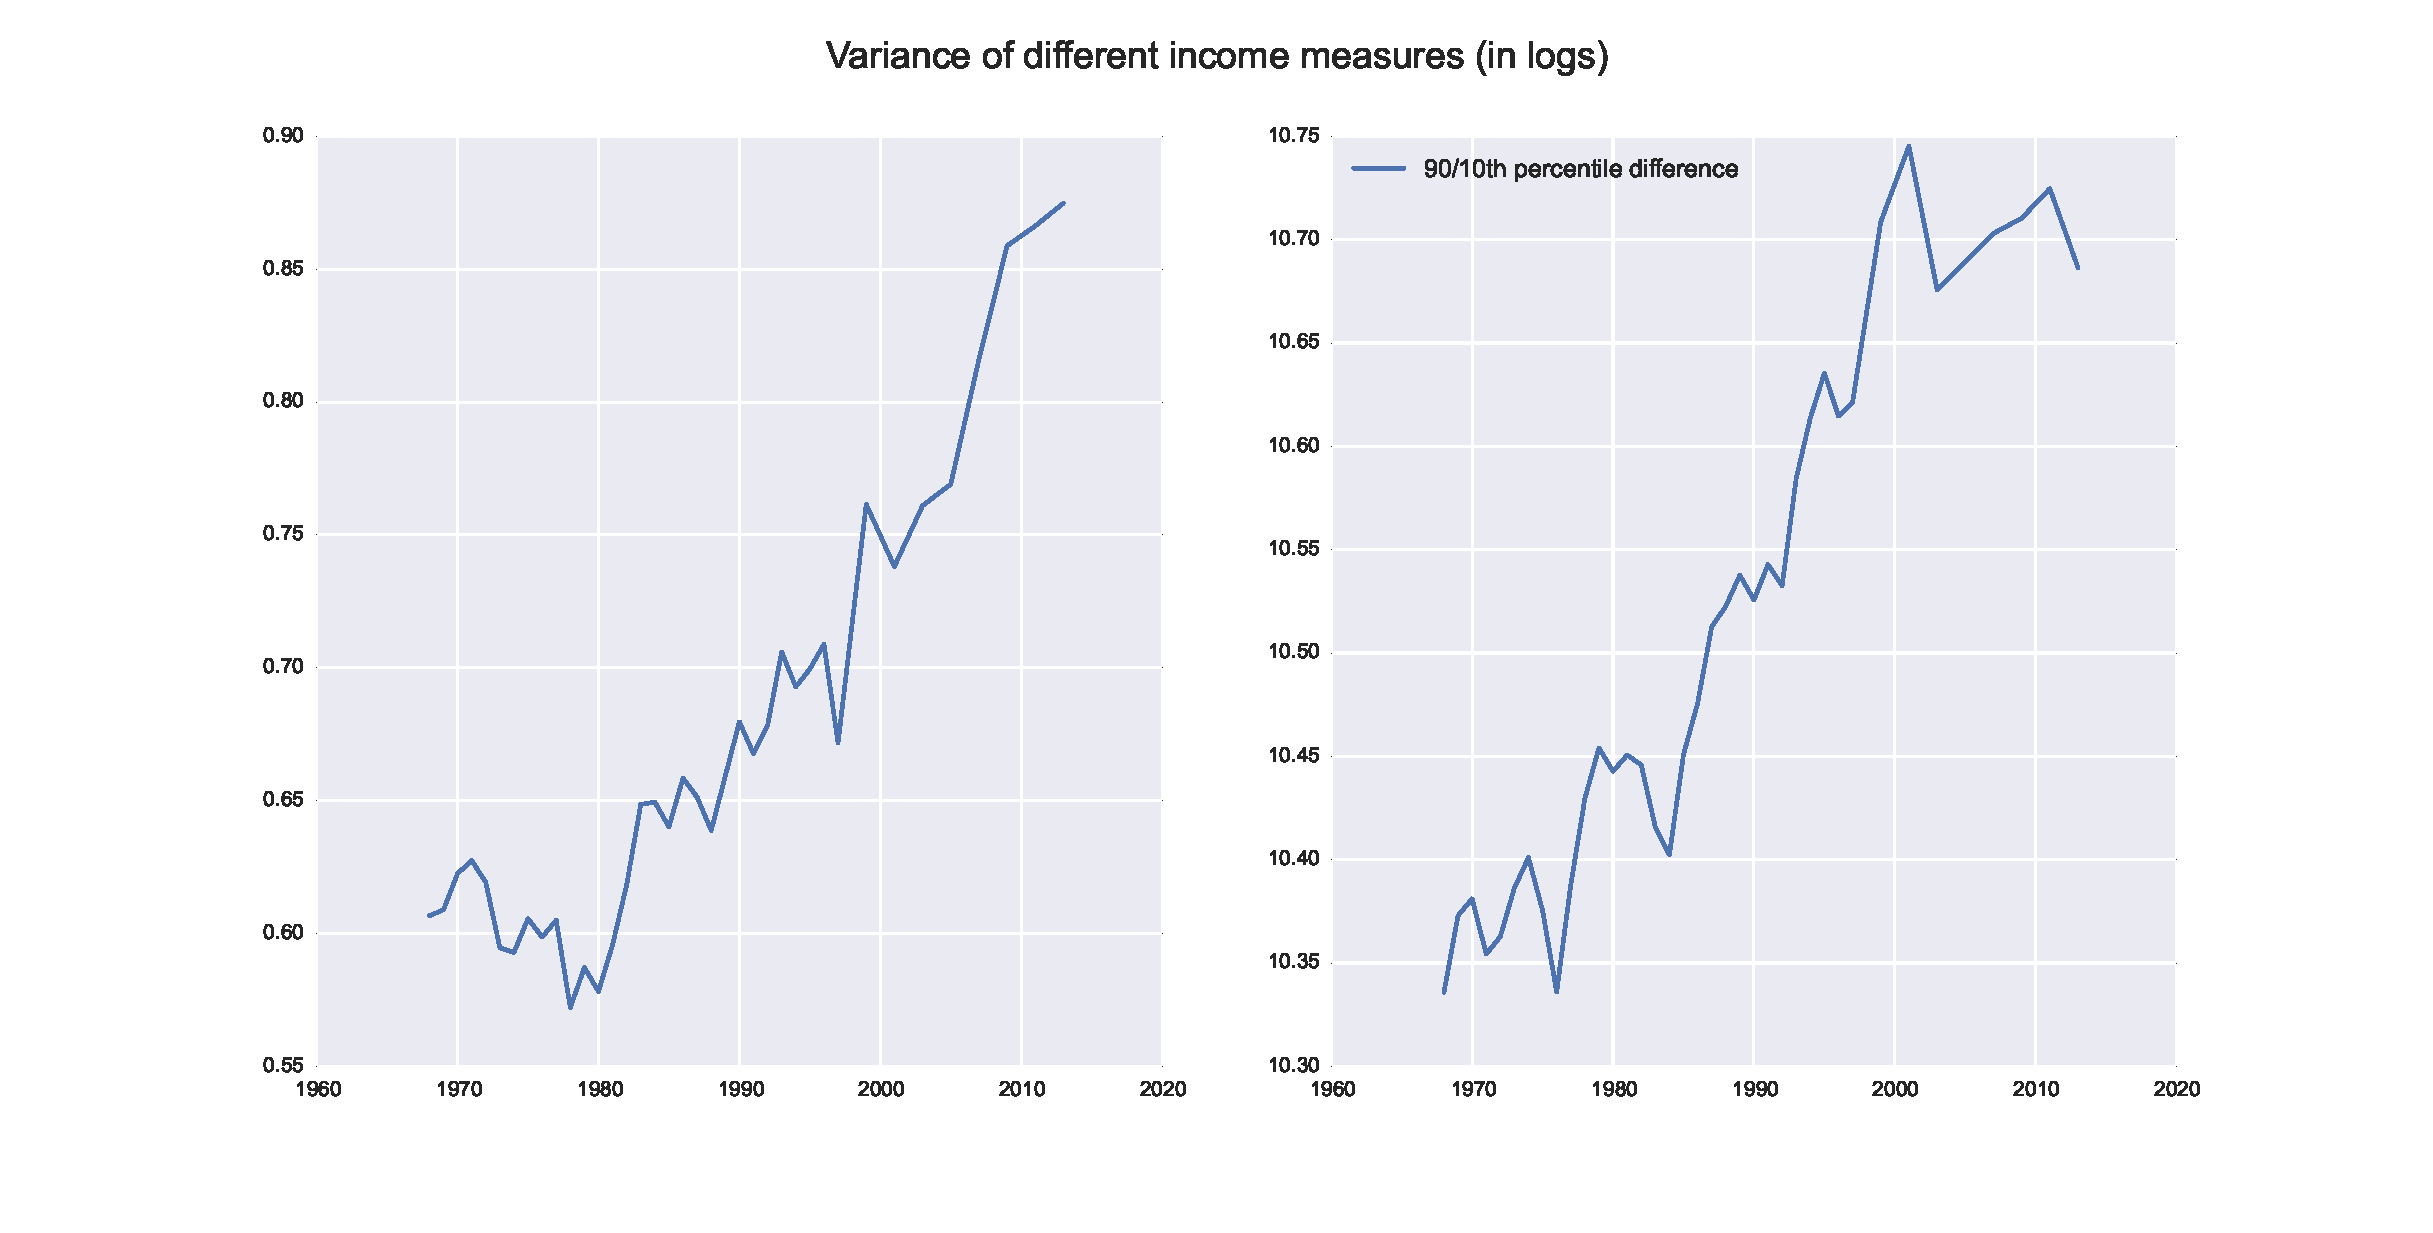
\includegraphics[width=\columnwidth]{PSID_incvar}
\caption{Variance of log income and 90/10 percentile width for our sample of
BHPS households}
\label{fig:psid_incvar}
\end{figure}

\begin{figure}
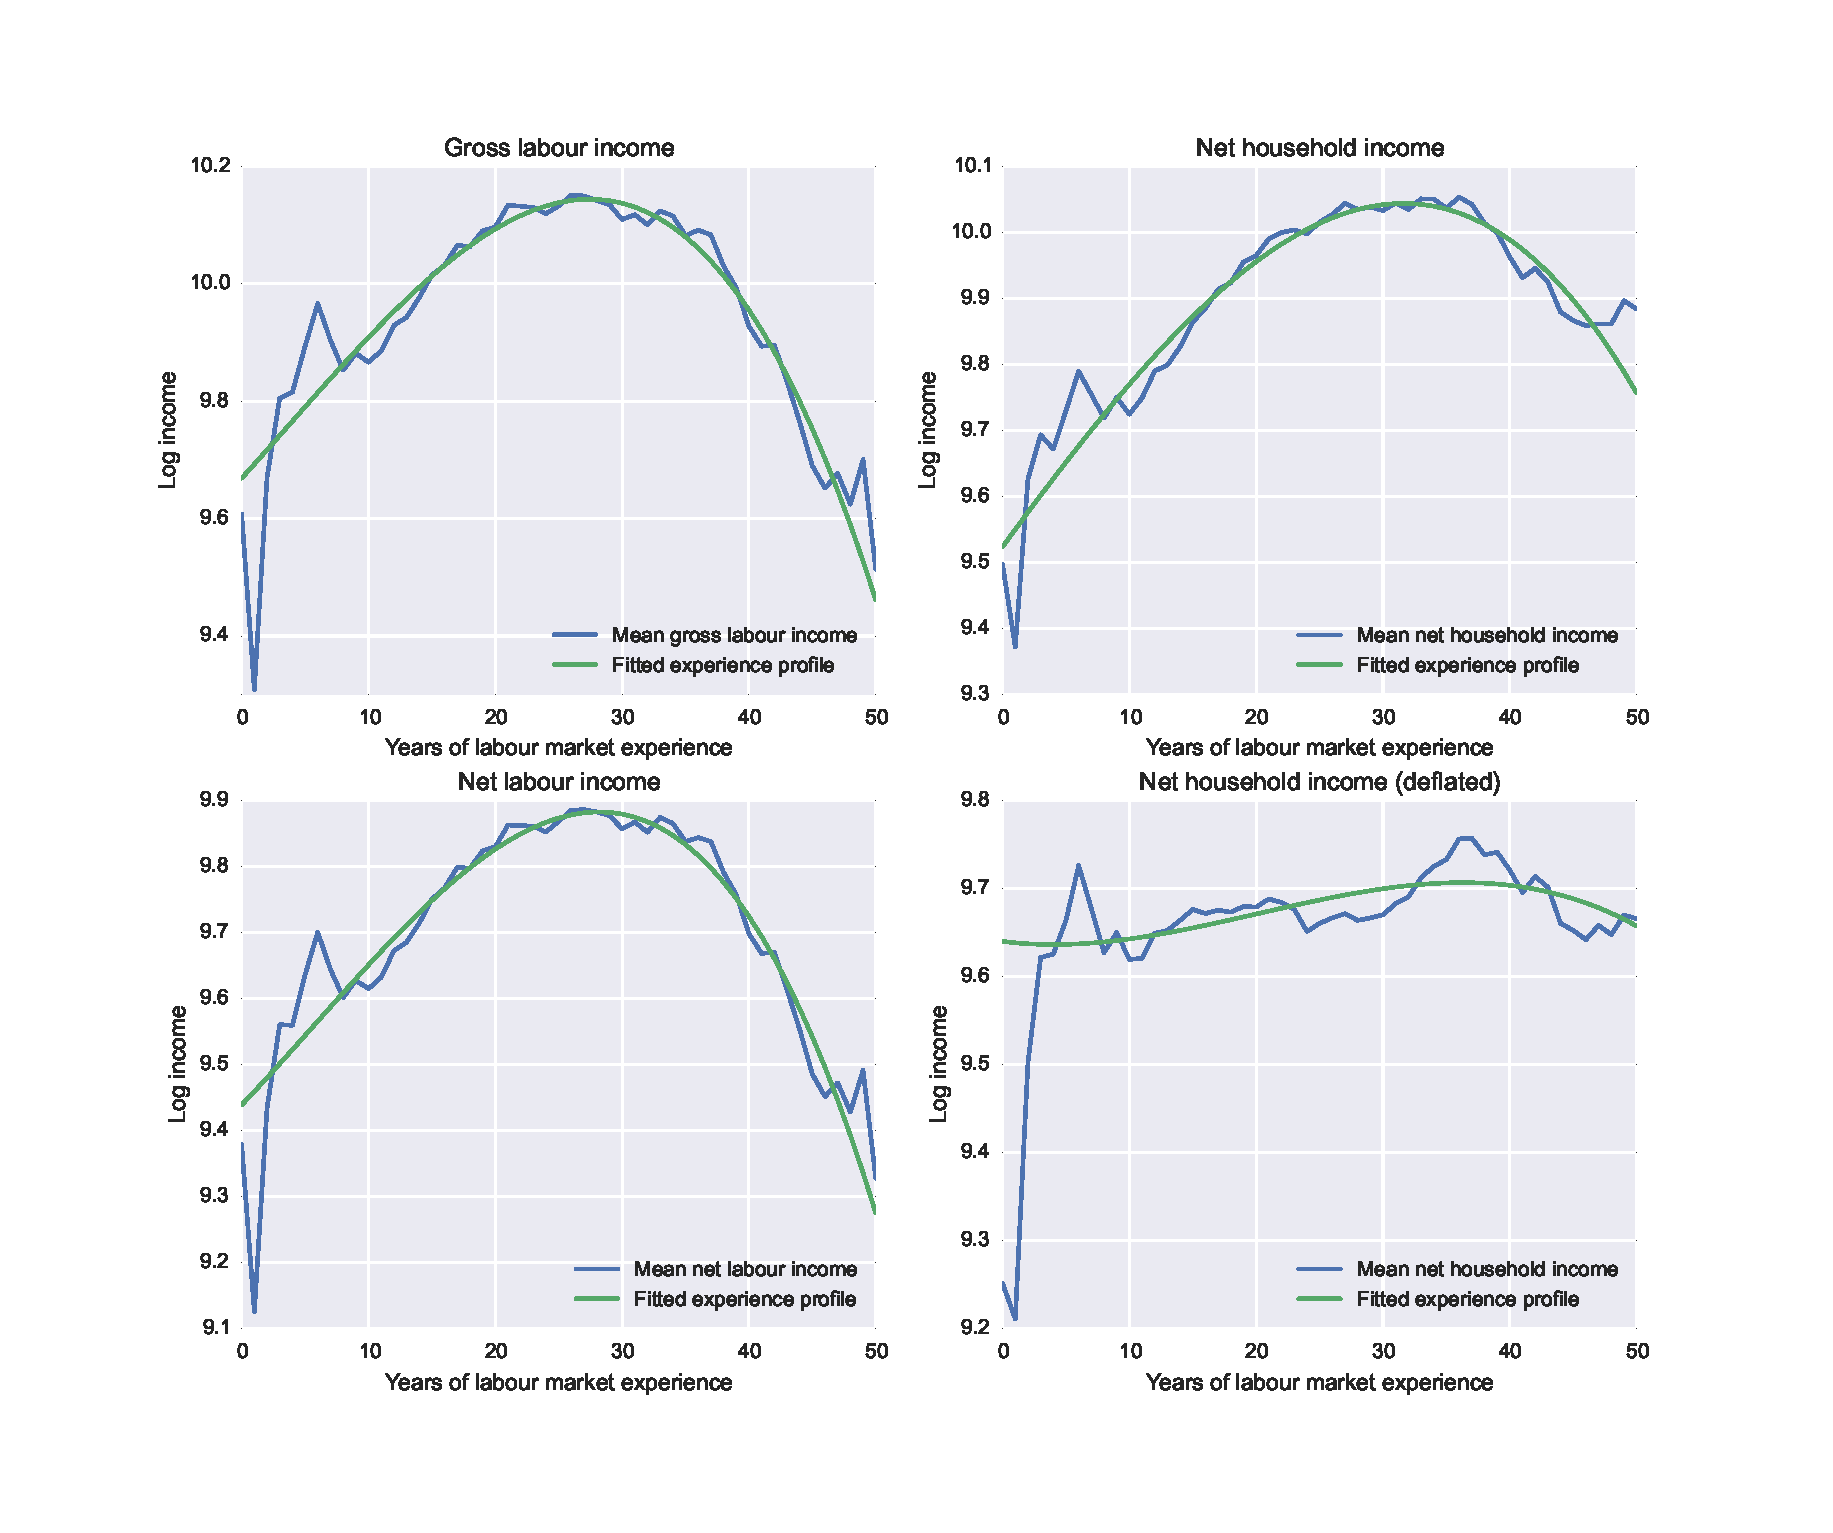
\includegraphics[width=\columnwidth]{BHPS_fitted_profiles}
\caption{Log mean income and fitted experience profiles for the BHPS 1992 
-- 2009}
\label{fig:bhps_profiles}
\end{figure}




\section{Results}
Table \ref{tab:BHPS_results} shows the results of estimating both RIP and HIP
processes on our sample of households from the BHPS, using the four different
income measures described previously. The results are largely unsurprising 
qualitatively, with the variance of persistent shocks declining from 0.1 for
the most volatile process (gross labour earnings) to 0.07 for net labour earnings,
to 0.027 for net household income. A similar pattern can be observed for the 
transitory shock, declining from 0.08 to 0.07 and 0.056, respectively. The 
estimates for the main parameter of interest, the cross-sectional dispersion 
in individual specific growth rates $\beta^i$ behaves accordingly, dropping from 
0.00032 (consistent with the findings for the main PSID sample in 
\citet{Guvenen2009}), to 0.00019 and 0.00011. Interestingly, some of the decrease
in the parameters that increase cross-sectional dispersion over the life-cycle
of a cohort is offset by a rise in the cross-sectional inequality in intercepts, 
$\var_{\alpha}$ rises from 0.036 in the gross labour income sample to 0.052 in 
the net household income sample. The persistence of 

\begin{table}%
\begin{tabular}{l|cccccc}
                     &$\rho$ & $\sigma^2_{\eta}$&$\sigma^2_{\varepsilon}$&$\sigma^2_{\alpha}$&$\sigma^2_{\beta}$&$\sigma_{\alpha \beta}$\\
\hline
\hline
\multicolumn{7}{c}{Restricted income process: $\sigma^2_{\beta} \stackrel{!}{=} 0$} \\
\hline \\
Gross labour income   & 0.925 &  0.045           &   0.135                &       0.0         &        --        &        --             \\
Net labour income     & 0.867 &  0.065           &   0.077                &       0.017       &        --        &        --             \\
Net household income  & 0.921 &  0.026           &   0.046                &       0.012       &        --        &        --             \\
Net household income (deflated) & 0.817 &  0.038 &   0.038                &       0.084       &        --        &        --             \\
\hline
\multicolumn{7}{c}{Heterogeneous income process; $\sigma^2_{\beta}$ unrestricted} \\
\hline
Gross labour income   & 0.719 &  0.106           &   0.080                &       0.036       &     0.00032      &       -0.51           \\
Net labour income     & 0.808 &  0.073           &   0.070                &       0.032       &     0.00019      &       -0.59           \\
Net household income  & 0.857 &  0.027           &   0.056                &       0.052       &     0.00011      &       -0.42           \\
Net household income (deflated) & 0.812 &  0.039 &   0.042                &       0.100       &        0.0       &       -1.0            \\
\hline
\end{tabular}
\caption{Results for the PSID sample 1968-1996; Guvenen (2009) refers to published results, Guvenen Matlab to results obtained by running
the code available on the journal website, short sample to my own estimation with the 1968-1996 data, full sample to the 1968-2013 data.}
\label{tab:BHPS_results}
\end{table}

\begin{table}%
\begin{tabular}{l|cccccc}
                       &$\rho$ & $\sigma^2_{\eta}$&$\sigma^2_{\varepsilon}$&$\sigma^2_{\alpha}$&$\sigma^2_{\beta}$&$\sigma_{\alpha \beta}$\\
\hline
\hline
\multicolumn{7}{c}{Restricted income process: $\sigma^2_{\beta} \stackrel{!}{=} 0$} \\
\hline \\
PSID, 1968--1986      & 0.960 &  0.015           &   0.061                &       0.058       &        --        &        --             \\
                &\footnotesize{(NaN)}&\footnotesize{(NaN)}&\footnotesize{(NaN)}& \footnotesize{(NaN)} &          &                       \\
PSID, 1987--2013      & 0.939 &  0.017           &   0.095                &       0.110       &        --        &        --             \\
                &\footnotesize{(NaN)}&\footnotesize{(NaN)}&\footnotesize{(NaN)}& \footnotesize{(NaN)} &          &                       \\
\hline
\multicolumn{7}{c}{Heterogeneous income process: $\sigma^2_{\beta}$ unrestricted} \\
\hline
PSID, 1968--1986      & 0.885 &  0.013           &   0.043                &       0.110       &      0.00001     &      -0.42            \\
           & \footnotesize{(6.19)}  & \footnotesize{(3.016)}& \footnotesize{(0.322)} & \footnotesize{(0.0)}&\footnotesize{(6.74)}  & \footnotesize{(954596.4)}    \\
PSID, 1987--2013      & 0.854 &  0.032           &   0.085                &       0.097       &      0.00025     &      -0.31            \\
           & \footnotesize{(7.99)}  & \footnotesize{(170084.7)}& \footnotesize{(0.854)} & \footnotesize{(512842.6)}&\footnotesize{(656.74)}  & \footnotesize{(954596.4)}    \\
\hline-
\end{tabular}
\caption{Results for PSID subsamples 1968 to 1986 and 1987 to 2013}
\label{tab:psid_subsample}
\end{table}

\begin{table}%
\begin{tabular}{l|cccccc}
                    &$\rho$ & $\sigma^2_{\eta}$&$\sigma^2_{\varepsilon}$&$\sigma^2_{\alpha}$&$\sigma^2_{\beta}$&$\sigma_{\alpha \beta}$\\
\hline
\hline 
\multicolumn{7}{c}{Restricted income process: $\sigma^2_{\beta} \stackrel{!}{=} 0$} \\
Guvenen (2009)   & 0.988 &  0.015           &   0.061                &       0.058       &        --        &        --             \\
Guvenen Matlab   & 0.935 &  0.010           &   0.023                &                   &        --        &        --             \\
1968-1996 sample & 0.932 &  0.010           &   0.036                &       0.084       &        --        &        --             \\
1968-2013 sample & 0.920 &  0.014           &   0.067                &       --          &        --        &        --             \\
\hline
\multicolumn{7}{c}{Heterogeneous income process: $\sigma^2_{\beta}$ unrestricted} \\
\hline
Guvenen (2009)   & 0.821 &  0.029           &   0.047                &   0.022           &     0.00038      &     --0.23            \\
Guvenen Matlab   & 0.853 &  0.013           &   0.030                &   0.030           &     0.00031      &     --0.30            \\
1968-1996 Sample & 0.907 &  0.010           &   0.058                &   0.036           &     0.00015      &       0.05            \\
1968-1996 Sample & 0.906 &  0.010           &   0.057                &   0.039           &     0.00015      &     --7.5e-6          \\
1968-1996 Sample & 0.903 &  0.010           &   0.056                &   0.046           &     0.00017      &     --0.11            \\
1968-1996 Sample & 0.903 &  0.010           &   0.056                &   0.046           &     0.00017      &     --0.11            \\
1968-2013 sample & 0.839 &  0.017           &   0.064                &   0.047           &     0.00026      &     --0.32            \\
\hline
\end{tabular}
\caption{Results for the BHPS sample 1992-2009, different income measures.}
\label{BHPS_results}
\end{table}
